\documentclass{article}
\usepackage{amsmath}
\usepackage{mathabx}
\usepackage{cancel}
\usepackage{fancyhdr}
\usepackage{graphicx}
\usepackage{hyperref}

\usepackage[top=1in, bottom=1in, left=1in, right=1in]{geometry}

\pagestyle{fancy}

%------------------------------------------------------
%	BEGIN DOCUMENT
%------------------------------------------------------

\begin{document}

%------------------------------------------------------
%	HEADER
%------------------------------------------------------

\fancyhead[LO,L]{AA214c}
\fancyhead[CO,C]{Final Project}
\fancyhead[RO,R]{Zachary del Rosario}

%------------------------------------------------------
%	CONTENT
%------------------------------------------------------

% -------------------------
\section{Introduction}
% -------------------------
This report details the design and performance of my viscous flow solver for AA214c. The code is available in a public GitHub repository, located at \url{https://github.com/zdelrosario/flow}.

% -------------------------
\section{Solver}
% -------------------------
This section details the design of the solver. The scheme is intended to find steady-state solutions to the full 2-D Navier-Stokes equations using a finite volume method with local time-stepping. The equations to be solved are

\begin{equation}
\begin{aligned}
\frac{\partial \rho}{\partial t} + \frac{\partial}{\partial x_i} \rho u_i &= 0, \\
\frac{\partial \rho u_i}{\partial t} + \frac{\partial}{\partial x_j}\left(\rho u_iu_j + P\delta_{ij} - \tau_{ij} \right) &= 0, \\
\frac{\partial \rho E}{\partial t} + \frac{\partial}{\partial x_i}\left(\rho u_i H + Q_i - \tau_{ij}u_j\right) &= 0,
\end{aligned}
\end{equation}

where $\tau_{ij}$ is the viscous stress tensor, $\rho E=\frac{P}{\gamma-1}+\frac{1}{2}\rho(u^2+v^2)$ is the internal energy, and $\rho H=\rho E+P$ is the internal enthalpy. The equations are solved in conservation form, which is expressed

\begin{equation}
\frac{\partial W}{\partial t} + \frac{\partial F(W)}{\partial x} + \frac{\partial G(W)}{\partial y} = 0,
\end{equation}

where

\begin{equation}
\begin{aligned}
W &= (\rho, \rho u, \rho v, \rho E)^T \\
F &= F_e + F_v \\
G &= G_e + G_v \\
F_e &= (\rho u, \rho u^2 + P, \rho uv, \rho u H)^T, \\
G_e &= (\rho v, \rho uv, \rho v^2 + P, \rho v H)^T, \\
F_v &= (0, \tau_{xx}, \tau_{xy}, Q_x-\tau_{xx}u-\tau_{xy}v)^T, \\
F_v &= (0, \tau_{xy}, \tau_{yy}, Q_y-\tau_{yy}v-\tau_{xy}u)^T.
\end{aligned}
\end{equation}

These equations are discretized in a finite volume scheme on a structured (cartesian) grid; the superscript $k$ denotes the time step, while the subscripts $i$ and $j$ denote the horizontal and vertical cell indices, respectively. Note that a whole index denotes a cell, while a half index (e.g. $i+1/2$) denotes a cell interface.

\subsection{Euler Fluxes}
These terms account for momentum and pressure effects, and are handled via the JST scheme. This is a central flux with an added artificial dissipation term to eliminate odd-even decoupling. The fluxes take the form

\begin{equation}
\begin{aligned}
F_{e,i+1/2,j}^{(k)} &= \frac{1}{2}(F_{e,i,j}^{(k)}+F_{e,i+1,j}^{(k)}) - \epsilon(|u_{i+1/2,j}^{(k)}|+c_{i+1/2,j}^{(k)})(W_{i+1,j}^{(k)}-W_{i,j}^{(k)}), \\
G_{e,i,j+1/2}^{(k)} &= \frac{1}{2}(F_{e,i,j}^{(k)}+F_{e,i,j+1}^{(k)}) - \epsilon(|u_{i,j+1/2}^{(k)}|+c_{i,j+1/2}^{(k)})(W_{i,j+1}^{(k)}-W_{i,j}^{(k)}),
\end{aligned}
\end{equation}

where $c$ is the local speed of sound. For the cases considered below, we use $\epsilon = 1/4$. The local rate of change is then given by

\begin{equation}
\begin{aligned}
\frac{\partial W^{(k)}_{i,j}}{\partial t} = -\frac{F_{e,i+1,j}^{(k)}-F_{e,i,j}^{(k)}}{\Delta x} -\frac{G_{e,i,j+1}^{(k)}-G_{e,i,j}^{(k)}}{\Delta y}.
\end{aligned}
\end{equation}

\subsection{Viscous Fluxes}
The viscous fluxes include not just the viscous terms, but all quantities which involve a second derivative of the flow variables -- these require different handling than a central flux. To compute second derivatives, we compute first derivatives on the corners of each cell via a local linear interpolant, using the surrounding cell values. These corners are averaged to find the values at the center of a cell interface; for example, on the right interface, the top right and bottom right corner values are averaged. The second derivative is then computed buy taking the difference of these interface values; for example, the second x-derivative is found by subtracting the value on the left interface from that on the right interface. This method is used to discretize the $F_v$ and $G_v$ terms.

\subsection{Time Stepping}
For time integration, the classical explicit RK4 scheme is employed, whose Butcher table is given below.

\begin{table} [!ht]
\centering
\begin{tabular}{c|cccc}
  0 & 0   &   0 &   0 &   0 \\
1/2 & 1/2 &   0 &   0 &   0 \\
1/2 & 0   & 1/2 &   0 &   0 \\
  1 & 0   &   0 &   1 &   0 \\
\hline
    & 1/6 & 1/3 & 1/3 & 1/6
\end{tabular}
\end{table}

The timestep is local, and based on a CFL estimate given by

\begin{equation}
\Delta t = \frac{\Delta x \Delta y}{(|u|+c)\Delta x + (|v|+c)\Delta y},
\end{equation}

where $\Delta x$ and $\Delta y$ are the x and y cell side lengths. For contorted cells, the x- and y-values are averaged.

\subsection{Boundary Conditions}
Boundary conditions are enforced weakly by setting ghost cell states. Walls are modeled using a no-slip condition, which is enforced by setting the ghost cell state to have the opposite velocities as the interior cell. Supersonic inflow and outflow conditions are handled simply using dirichlet and neumann conditions respectively; a supersonic inflow has all characteristics taking information from the free stream into the domain, while supersonic outflow has all characteristics flowing from the domain to the exterior.

Subsonic inflow and outflow conditions are modeled using characteristics; specifically, preserving Riemann invariants. The implementation below is based on the code PyFR. Let the subscript $L$ denote the interior state, and the subscript $R$ denote the exterior state. Let $(n_x,n_y)^T$ denote the cell normal, and define the projected velocities

\begin{equation}
\begin{aligned}
V_{n,L} &= u_Ln_x + v_Ln_y, \\
V_{n,R} &= u_Rn_x + v_Rn_y,
\end{aligned}
\end{equation}

the Riemann invariants and stared states are then

\begin{equation}
\begin{aligned}
R_L &= V_{n,L} + \frac{2}{\gamma-1}c_L, \\
R_R &= V_{n,R} - \frac{2}{\gamma-1}c_R, \\
c^* &= \frac{1}{4}(\gamma-1)(R_L-R_R), \\
u_n^* &= \frac{1}{2}(R_L+R_R).
\end{aligned}
\end{equation}

From this point, intermediate values are computed differently for inflow and outflow conditions. For an inflow condition, we compute

\begin{equation}
\begin{aligned}
s^{-1} &= \rho_{\infty}^{\gamma}/P_{\infty}, \\
u_R &= u_{\infty} + (u_n^*-V_{n,R})n_x, \\
v_R &= v_{\infty} + (u_n^*-V_{n,R})n_y,
\end{aligned}
\end{equation}

where the $\infty$ subscript denotes free stream conditions. For an outflow, we compute

\begin{equation}
\begin{aligned}
s^{-1} &= \rho_L^{\gamma}/P_L, \\
u_R &= u_L + (u_n^*-V_{n,L})n_x, \\
v_R &= v_L + (u_n^*-V_{n,L})n_y.
\end{aligned}
\end{equation}

Then the ghost state value is

\begin{equation}
\begin{aligned}
\rho_R &= [\frac{1}{\gamma}(s^{-1}c^*)]^{1/(\gamma-1)} \\
(\rho u)_R &= \rho_Ru_R \\
(\rho v)_R &= \rho_Rv_R \\
(\rho E)_R &= \frac{1}{\gamma-1}P_R + \frac{1}{2}\rho_R(u_R^2+v_R^2).
\end{aligned}
\end{equation}

\subsection{Convergence}
The Residual described below is defined as

\begin{equation}
\text{Res} = \left\|\frac{\partial W^{(k)}_{i,j}}{\partial t}\right\|_\infty,
\end{equation}

where the infinity-norm is computed over both spatial indices $i,j$ and states $W_1$ through $W_4$. This measure tells us that no state is changing at a rate greater than Res anywhere in the domain.

\newpage
% -------------------------
\section{Test Cases}
% -------------------------
\subsection{Flat Plate Boundary Layer}
Our first test case is an attempt to reproduce the classical result of a Blasius laminar boundary layer on a flat plate. The inlet state is given as

\begin{equation*}
W_{\infty} = (1.1462 \text{kg}/\text{m}^3,79.0076\text{kg}*\text{m}/\text{s},0\text{kg}*\text{m}/\text{s},3.4218\times10^5\text{J}/\text{m}^3)^T.
\end{equation*}

The left boundary is a subsonic inlet, the top and right subsonic outlets, and the bottom is a mixture of a symmetry condition (where the vertical momentum is mirrored) forward of the plate, and a wall condition modeling the plate. Results are shown in Figure \ref{fig:plate_contour} through \ref{fig:plate_convergence}. Fairly poor agreement is seen in both comparisons against the Blasius solution -- this is a major issue, but I've been unable to figure out what's wrong.

\begin{figure}[!ht]
\centering
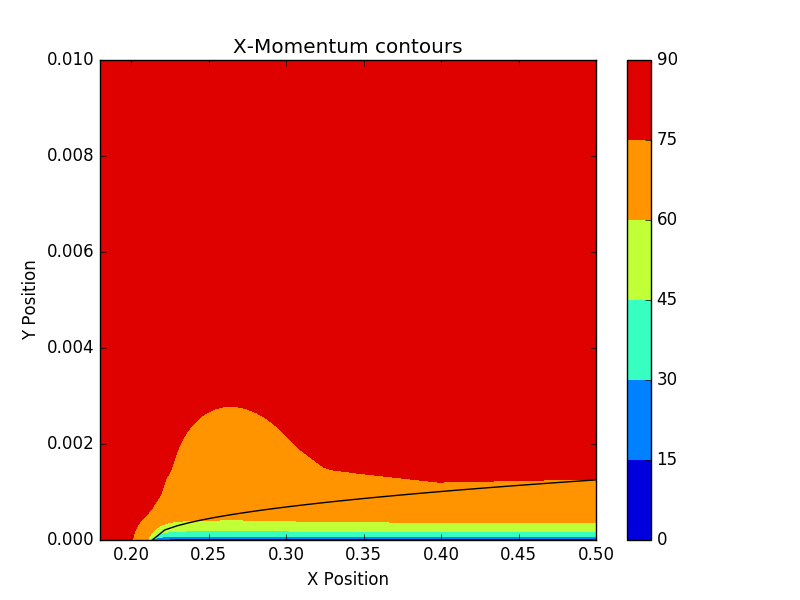
\includegraphics[width=0.7\textwidth]{images/plate_contour.png}
\caption{Momentum contours for flat plate test case. The Blasius profile is shown as a black line.}
\label{fig:plate_contour}
\end{figure}

\newpage
\begin{figure}[!ht]
\centering
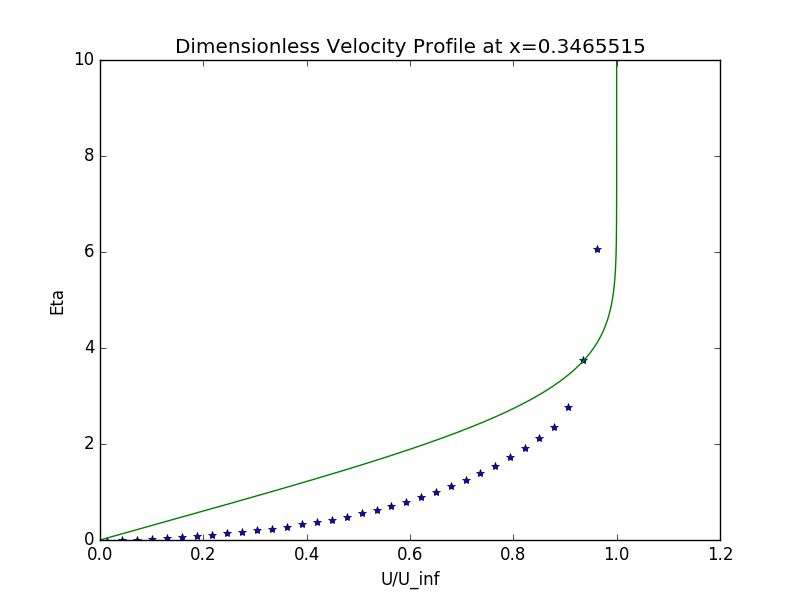
\includegraphics[width=0.7\textwidth]{images/plate_profile.png}
\caption{Comparison of Blasius velocity profile with numerical results.}
\label{fig:plate_profile}
\end{figure}

\begin{figure}[!ht]
\centering
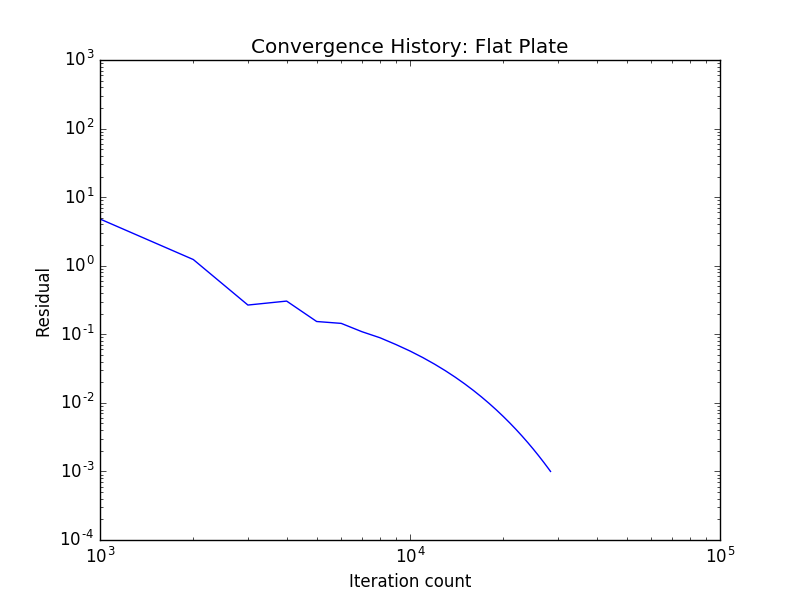
\includegraphics[width=0.7\textwidth]{images/plate_convergence.png}
\caption{Convergence history for Flat Plate test case.}
\label{fig:plate_convergence}
\end{figure}

\newpage
\subsection{Transonic Symmetric Airfoil}
This test case considers a $12\%$ thick bi-parabolic airfoil. The inlet state is given

\begin{equation*}
W_{\infty} = (1.1462 \text{kg}/\text{m}^3,1.5928\times10^2\text{kg}*\text{m}/\text{s},0\text{kg}*\text{m}/\text{s},5.9861\times10^4\text{J}/\text{m}^3)^T,
\end{equation*}

which corresponds to $M=0.9$ and $Re=9\times10^6$. A subsonic inlet is used for the left boundary, while the top and right boundaries are subsonic outlets. A symmetry condition is used for the bottom forward and aft of the airfoil, while the airfoil itself has a wall condition.

\begin{figure}[!ht]
\centering
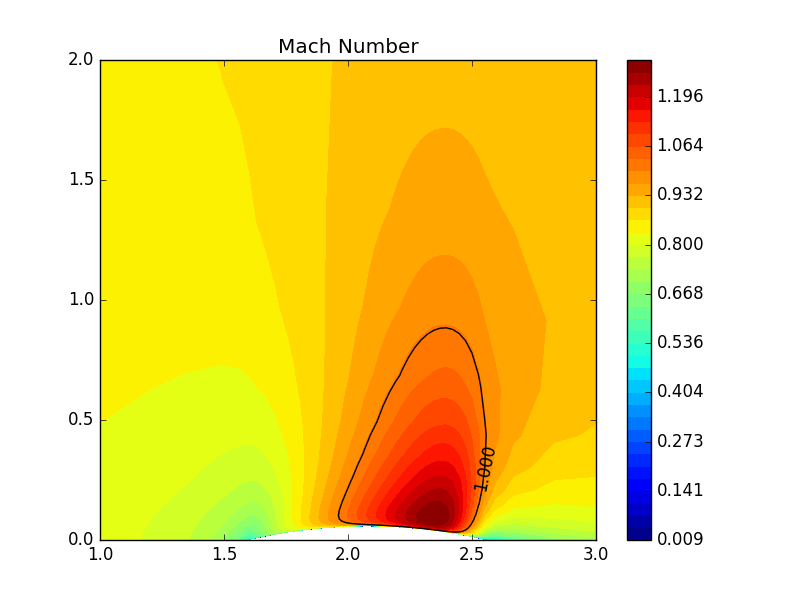
\includegraphics[width=0.7\textwidth]{images/airfoil_mach.png}
\caption{Mach contours for Symmetric Airfoil test case. The region of $M=1$ is marked with a black contour line. The low Mach values on and behind the trailing edge point toward a viscous wake -- this is likely to be quantitatively inaccurate based on the Flat Plate test case, but at least it is qualitatively correct.}
\label{fig:airfoil_mach}
\end{figure}

\begin{figure}[!ht]
\centering
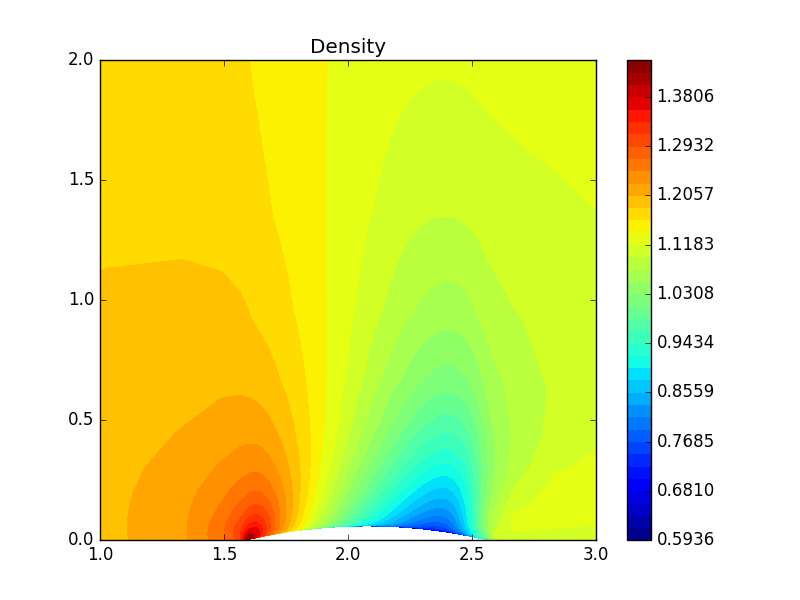
\includegraphics[width=0.7\textwidth]{images/airfoil_density.png}
\caption{Density contours for Symmetric Airfoil test case. }
\label{fig:airfoil_density}
\end{figure}

\begin{figure}[!ht]
\centering
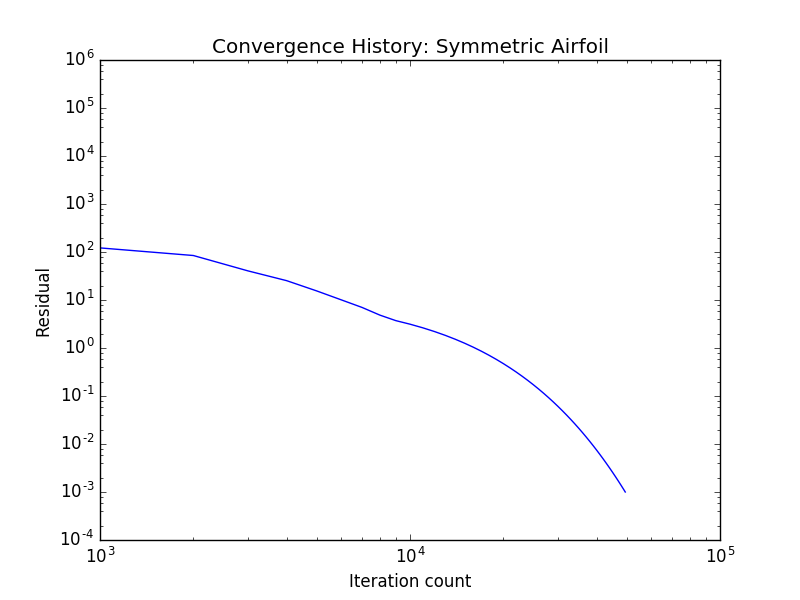
\includegraphics[width=0.7\textwidth]{images/airfoil_convergence.png}
\caption{Convergence history for Symmetric Airfoil test case.}
\label{fig:airfoil_convergence}
\end{figure}

Integrating the pressure gives a drag coefficient of $C_d = 0.00028$, which seems like a sever underprediction. This is unsurprising, given that the boundary layer is significantly thinner than it should be.

\newpage
% -------------------------
\section{Conclusion}
% -------------------------
Overall, I am rather unhappy with my solver's performance. The solver is unable to reproduce classical results in simple test cases, and therefore is useless for the purposes of analysis. I believe many of my issues stem from choosing to implement in C++, a language I am not very comfortable with. I had hoped to gain some speed benefit from implementing in a low-level language, but this was offset in terms of development time, as I spent an unacceptably long period of time solving CS problems, rather than solving numerical issues. Ultimately, I spent weeks trying to debug my fluxes, all to no avail. Unfortunately, I need to turn in this half-finished solver, and move on with my life.

\end{document}